\documentclass[12pt, twoside]{article}
\usepackage[letterpaper, margin=1in, headsep=0.5in]{geometry}
\usepackage[english]{babel}
\usepackage[utf8]{inputenc}
\usepackage{amsmath}
\usepackage{amsfonts}
\usepackage{amssymb}
\usepackage{tikz}
%\usetikzlibrary{quotes, angles}

\usepackage{graphicx}
\usepackage{enumitem}
\usepackage{multicol}

\usepackage{fancyhdr}
\pagestyle{fancy}
\fancyhf{}
\renewcommand{\headrulewidth}{0pt} % disable the underline of the header

\fancyhead[RE]{\thepage}
\fancyhead[RO]{\thepage \\ Name: \hspace{3cm}}
\fancyhead[L]{BECA / Dr. Huson / 10th Grade Geometry\\* Unit 11: Analytic Geometry Review\\22 May 2019}

\begin{document}
\subsubsection*{Homework: Point-slope and linear equations}
  \begin{enumerate}

  \item Write down the slope perpendicular to the given slope. \vspace{0.5cm}
    \begin{enumerate}
      \begin{multicols}{2}
      \item   $m=\frac{1}{2} \hspace{1cm} m_{\perp} = $ \vspace{1cm}
      \item   $m= -3 \hspace{1cm} m_{\perp} = $
      \item   $m= 2 \hspace{1cm} m_{\perp} = $ \vspace{1cm}
      \item   $m= -\frac{3}{2} \hspace{1cm} m_{\perp} = $
      \end{multicols}
    \end{enumerate}

  \item Write down the center and radius of each circle.
    \begin{enumerate}
      \begin{multicols}{2}
      \item   $(x-4)^2+(y-2)^2=25$
      \item   $(x+1)^2+(y-5)^2=16^2$
      \end{multicols}
    \end{enumerate}  \vspace{2cm}

  In the following problems, use the point-slope formula: $y-y_1=m (x-x_1)$
    \item What is the equation of a line through $(1,2)$ with slope $m=2$?  \vspace{2cm}
    \item What is the equation of a line through $(-5,3)$ parallel to the line $y=\frac{1}{2}x-2$?  \vspace{2cm}

    \item What is an equation of a line which passes through $(6,9)$ and is perpendicular to the line whose equation is $4x-6y=15$? \vspace{1cm}


    \newpage

      \item On the set of axes below, graph the quadrilateral $ABCD$ having coordinates $A(-3,-3)$, $B(5,1)$, $C(6,8)$, and $D(-2,4)$.
        \begin{center} %4 quadrant regents grid
        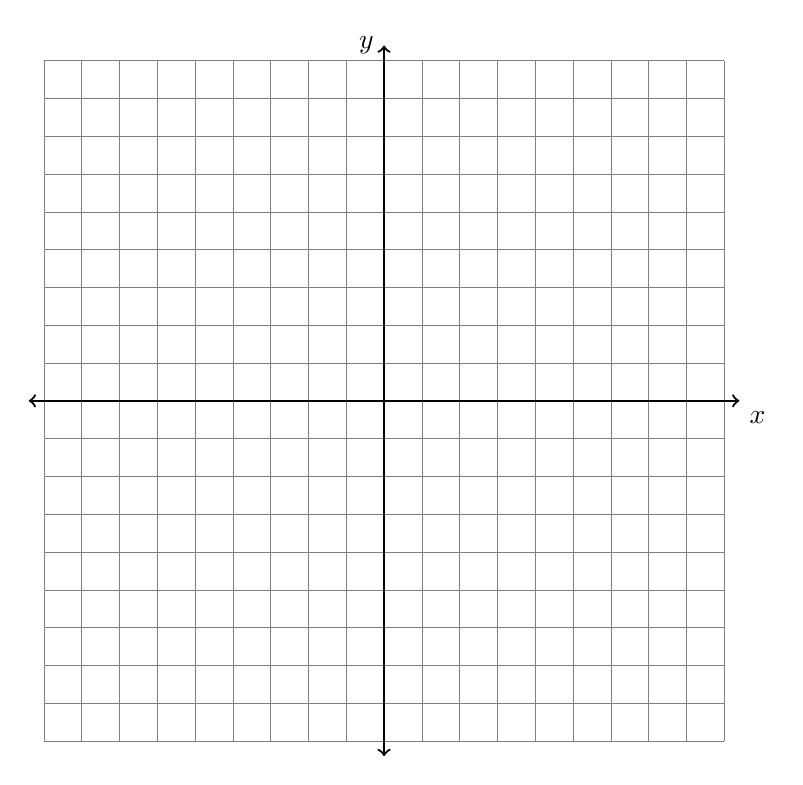
\begin{tikzpicture}[scale=.48]
          \draw [help lines] (-9,-9) grid (9,9);
          \draw [thick, <->] (-9.4,0) -- (9.4,0) node [below right] {$x$};
          \draw [thick, <->] (0,-9.4)--(0,9.4) node [left] {$y$};
          %\draw [thick] (-3,-3) node[below] {$A$}--
          %(5,1) node[right] {$B$}--
          %(6,8) node[left] {$C$}--
          %(-2,4) node[left] {$D$}--cycle;
          %\draw [fill] (5,0) circle [radius=0.1] node[above left] {$P$};
        \end{tikzpicture}
        \end{center}
        Find the length of each side of the quadrilateral.


  \end{enumerate}
\end{document}
